% Canonical caption for figCourseGradients.pdf
% Generated by: code/paper0/course_gradient_figure.py from
% mart.course_poverty (GATEWAY; code/ingest/crdc_courses.py).
% Regenerate: python code/paper0/course_gradient_figure.py
\begin{figure}[tbp]
  \centering
  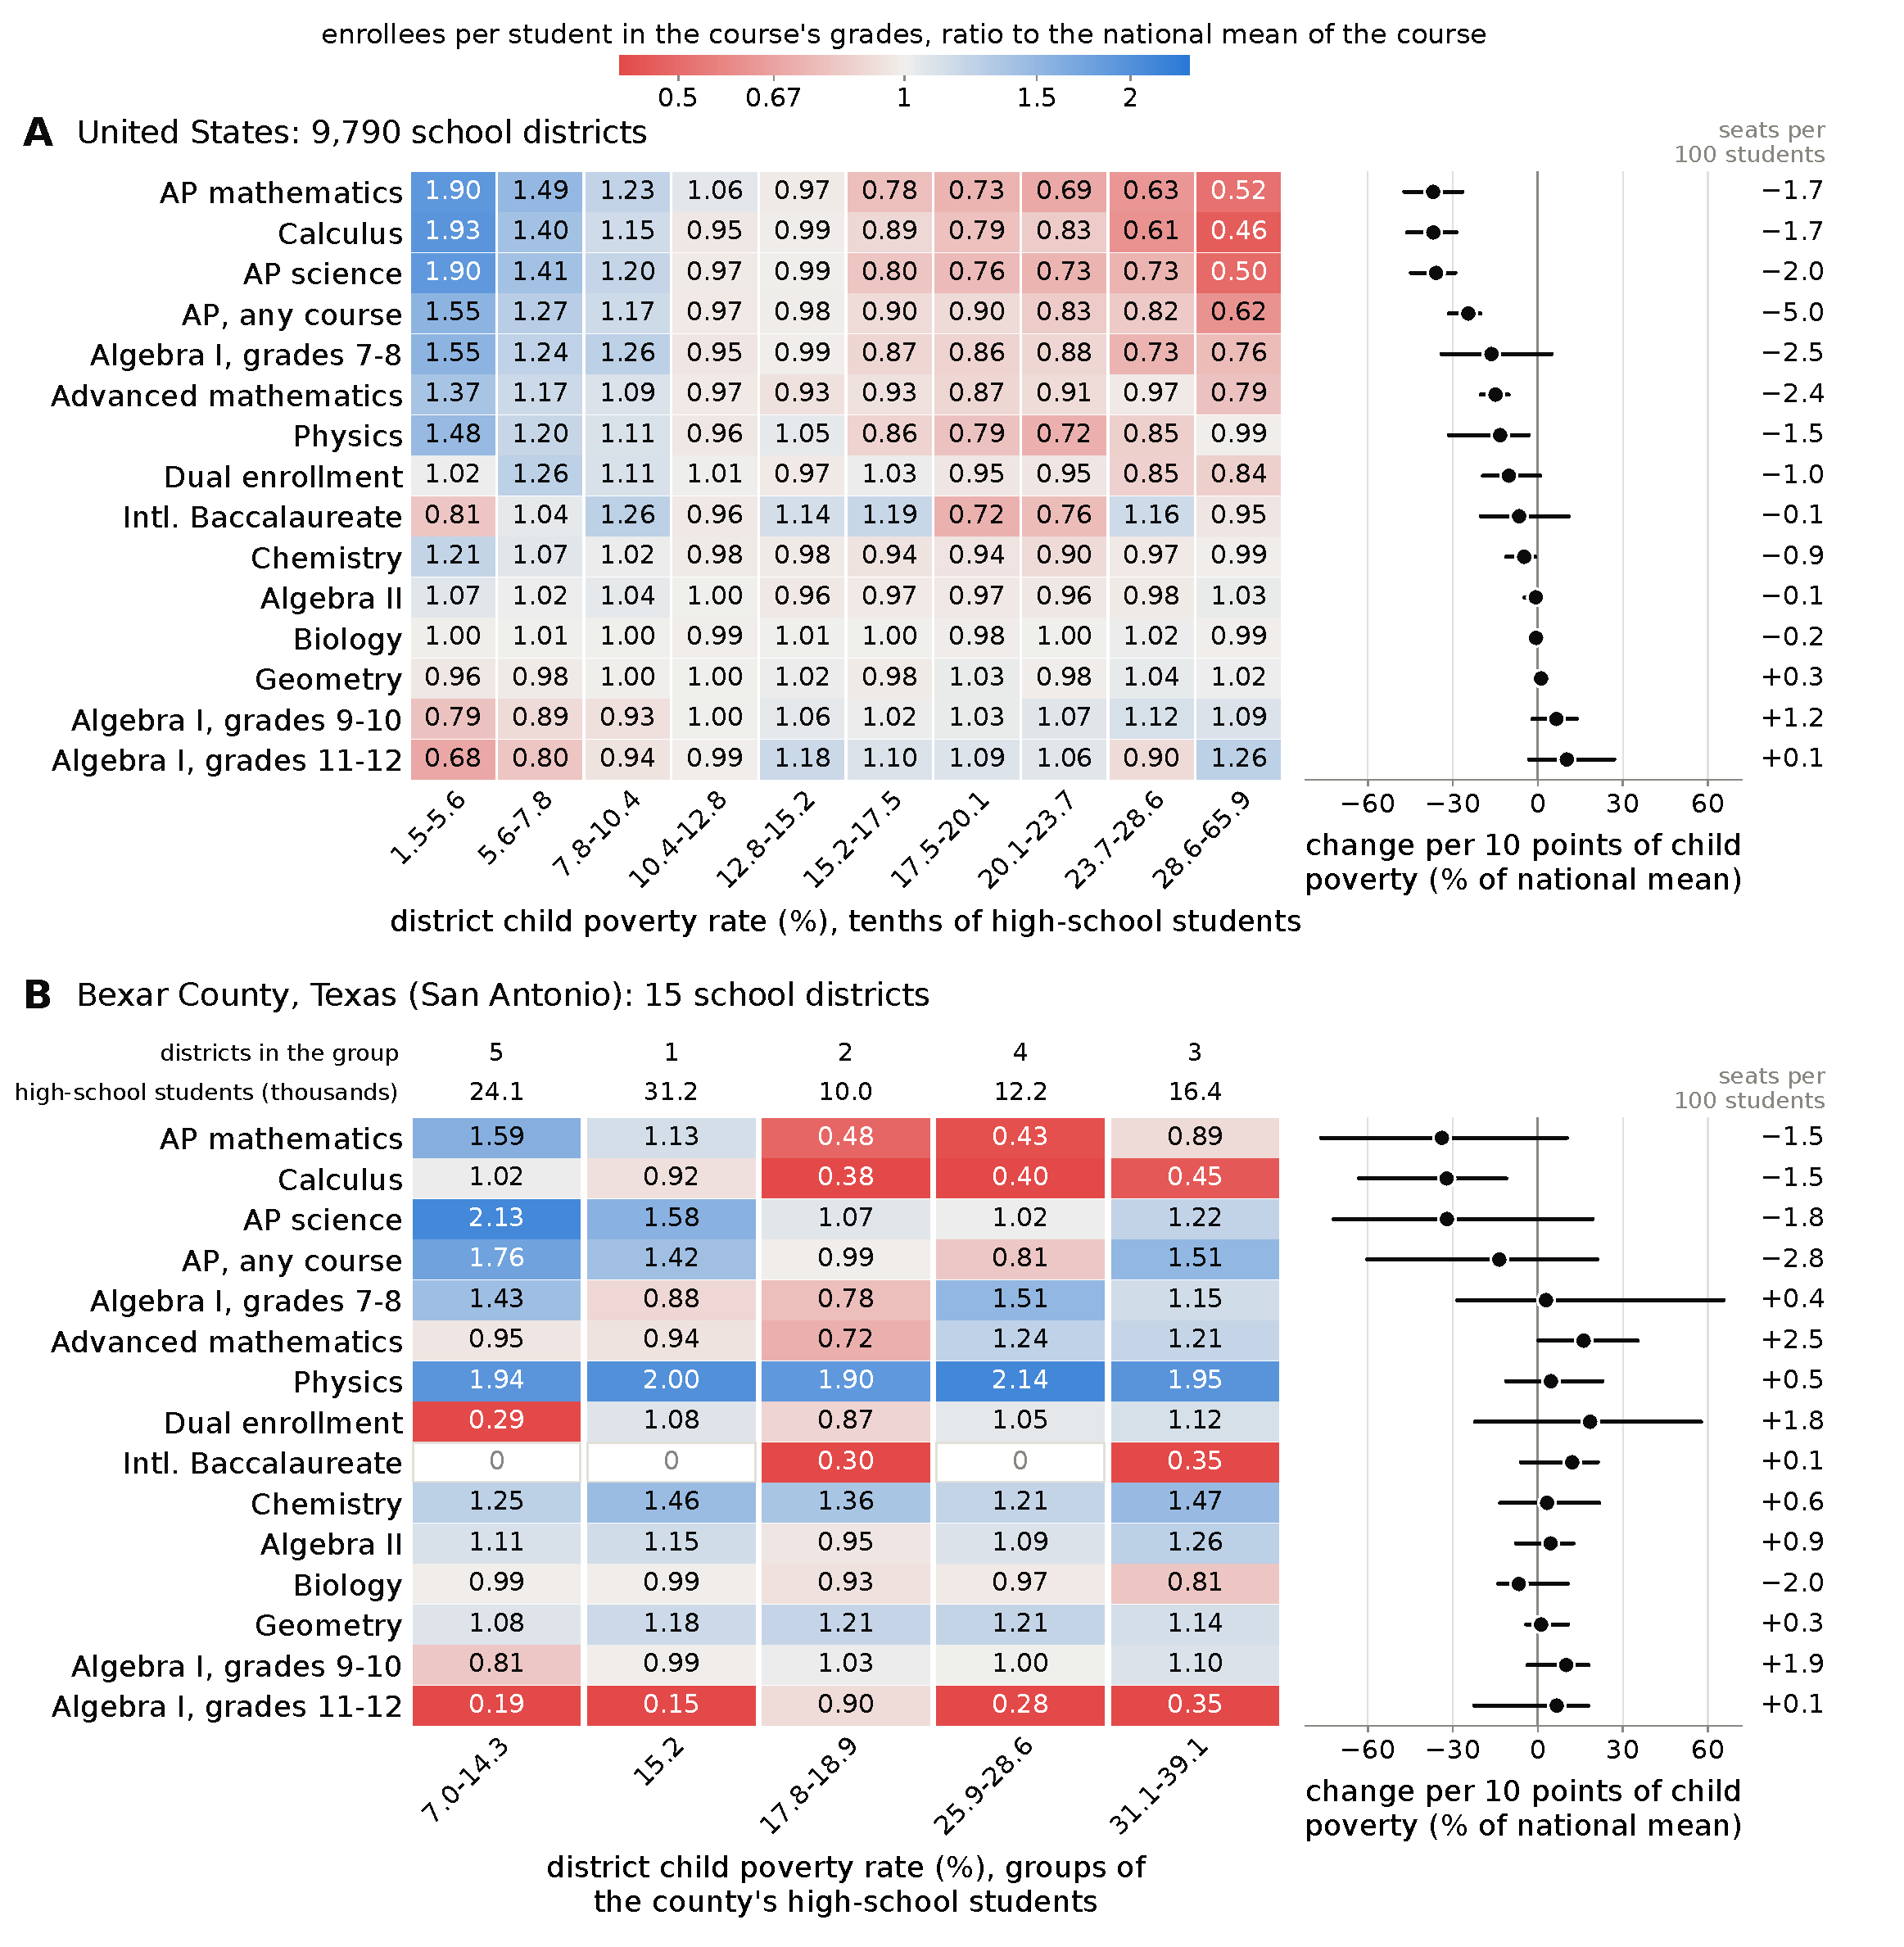
\includegraphics[width=0.92\textwidth]{figCourseGradients.pdf}
  \caption{Course enrollment and district child poverty, by
    course family (CRDC 2017--18; SAIPE 2017). Each count is
    divided by estimated enrollment in the grades of the course
    (grades 9--12, or grades 7 and 8 for Algebra~I in grades
    7--8), and each cell is the ratio of that rate to the
    national rate of the same course (1.00 is the national rate;
    blue above, red below; logarithmic color scale). (A) United
    States, the 9,790 districts of
    Figure~\ref{figCalculusPanels}. Left: tenths of high-school
    students ordered by district child poverty. Right: the
    weighted least-squares slope of the rate on child poverty,
    in percent of the national mean per ten percentage points of
    child poverty, with 95\% intervals from a state-cluster
    bootstrap (5,000 resamples); the numbers at the right
    restate each slope in enrollees per 100 students. Rows are
    ordered by this gradient in both panels. (B) The same
    display for the 15 school districts of Bexar County,
    Texas. The districts are ordered by child poverty and merged
    into 5 groups that each hold at least a tenth of the
    county's high-school students.
    The slope is computed over the 15 districts, with 95\%
    intervals from a bootstrap that resamples districts. A
    cell marked 0 reports no enrollment. Districts are the
    units; enrollment counts seats within one cycle, with no
    completion or outcome content.}
  \label{figCourseGradients}
\end{figure}
